% This is "sig-alternate.tex" V2.0 May 2012
% This file should be compiled with V2.5 of "sig-alternate.cls" May 2012
%
% This example file demonstrates the use of the 'sig-alternate.cls'
% V2.5 LaTeX2e document class file. It is for those submitting
% articles to ACM Conference Proceedings WHO DO NOT WISH TO
% STRICTLY ADHERE TO THE SIGS (PUBS-BOARD-ENDORSED) STYLE.
% The 'sig-alternate.cls' file will produce a similar-looking,
% albeit, 'tighter' paper resulting in, invariably, fewer pages.
%
% ----------------------------------------------------------------------------------------------------------------
% This .tex file (and associated .cls V2.5) produces:
%       1) The Permission Statement
%       2) The Conference (location) Info information
%       3) The Copyright Line with ACM data
%       4) NO page numbers
%
% as against the acm_proc_article-sp.cls file which
% DOES NOT produce 1) thru' 3) above.
%
% Using 'sig-alternate.cls' you have control, however, from within
% the source .tex file, over both the CopyrightYear
% (defaulted to 200X) and the ACM Copyright Data
% (defaulted to X-XXXXX-XX-X/XX/XX).
% e.g.
% \CopyrightYear{2007} will cause 2007 to appear in the copyright line.
% \crdata{0-12345-67-8/90/12} will cause 0-12345-67-8/90/12 to appear in the copyright line.
%
% ---------------------------------------------------------------------------------------------------------------
% This .tex source is an example which *does* use
% the .bib file (from which the .bbl file % is produced).
% REMEMBER HOWEVER: After having produced the .bbl file,
% and prior to final submission, you *NEED* to 'insert'
% your .bbl file into your source .tex file so as to provide
% ONE 'self-contained' source file.
%
% ================= IF YOU HAVE QUESTIONS =======================
% Questions regarding the SIGS styles, SIGS policies and
% procedures, Conferences etc. should be sent to
% Adrienne Griscti (griscti@acm.org)
%
% Technical questions _only_ to
% Gerald Murray (murray@hq.acm.org)
% ===============================================================
%
% For tracking purposes - this is V2.0 - May 2012

\documentclass{sig-alternate}
\usepackage[normalem]{ulem}

\begin{document}
%
% --- Author Metadata here ---
\conferenceinfo{WOODSTOCK}{'97 El Paso, Texas USA}
%\CopyrightYear{2007} % Allows default copyright year (20XX) to be over-ridden - IF NEED BE.
%\crdata{0-12345-67-8/90/01}  % Allows default copyright data (0-89791-88-6/97/05) to be over-ridden - IF NEED BE.
% --- End of Author Metadata ---

\title{Identifying minimal failure-inducing schemas for multiple faults\titlenote{(Does NOT produce the permission block, copyright information nor page numbering). For use with ACM\_PROC\_ARTICLE-SP.CLS. Supported by ACM.}}
\subtitle{[Extended Abstract]
\titlenote{A full version of this paper is available as
\textit{Author's Guide to Preparing ACM SIG Proceedings Using
\LaTeX$2_\epsilon$\ and BibTeX} at
\texttt{www.acm.org/eaddress.htm}}}
%
% You need the command \numberofauthors to handle the 'placement
% and alignment' of the authors beneath the title.
%
% For aesthetic reasons, we recommend 'three authors at a time'
% i.e. three 'name/affiliation blocks' be placed beneath the title.
%
% NOTE: You are NOT restricted in how many 'rows' of
% "name/affiliations" may appear. We just ask that you restrict
% the number of 'columns' to three.
%
% Because of the available 'opening page real-estate'
% we ask you to refrain from putting more than six authors
% (two rows with three columns) beneath the article title.
% More than six makes the first-page appear very cluttered indeed.
%
% Use the \alignauthor commands to handle the names
% and affiliations for an 'aesthetic maximum' of six authors.
% Add names, affiliations, addresses for
% the seventh etc. author(s) as the argument for the
% \additionalauthors command.
% These 'additional authors' will be output/set for you
% without further effort on your part as the last section in
% the body of your article BEFORE References or any Appendices.

\numberofauthors{8} %  in this sample file, there are a *total*
% of EIGHT authors. SIX appear on the 'first-page' (for formatting
% reasons) and the remaining two appear in the \additionalauthors section.
%
\author{
% You can go ahead and credit any number of authors here,
% e.g. one 'row of three' or two rows (consisting of one row of three
% and a second row of one, two or three).
%
% The command \alignauthor (no curly braces needed) should
% precede each author name, affiliation/snail-mail address and
% e-mail address. Additionally, tag each line of
% affiliation/address with \affaddr, and tag the
% e-mail address with \email.
%
% 1st. author
\alignauthor
Xintao Niu\\
       \affaddr{State Key Laboratory for Novel Software Technology}\\
       \affaddr{Nanjing University}\\
       \affaddr{China, 210093}\\
       \email{niuxintao@smail.nju.edu.cn}
% 2nd. author
\alignauthor
Changhai Nie\\
       \affaddr{State Key Laboratory for Novel Software Technology}\\
       \affaddr{Nanjing University}\\
       \affaddr{China, 210093}\\
       \email{changhainie@nju.edu.cn}
% 3rd. author
\alignauthor Alvin Chain\\
       \affaddr{Department of computing}\\
       \affaddr{Hong Kong Polytechnic University}\\
       \affaddr{Hong Kong}\\
       \email{cstschan@comp.polyu.edu.hk}
}
% There's nothing stopping you putting the seventh, eighth, etc.
% author on the opening page (as the 'third row') but we ask,
% for aesthetic reasons that you place these 'additional authors'
% in the \additional authors block, viz.
\additionalauthors{Additional authors: John Smith (The Th{\o}rv{\"a}ld Group,
email: {\texttt{jsmith@affiliation.org}}) and Julius P.~Kumquat
(The Kumquat Consortium, email: {\texttt{jpkumquat@consortium.net}}).}
\date{30 July 1999}
% Just remember to make sure that the TOTAL number of authors
% is the number that will appear on the first page PLUS the
% number that will appear in the \additionalauthors section.
\maketitle
\begin{abstract}
Minimal failure-inducing schema(MFS) is a important concept in combinatorial testing that indicate the failure-inducing interaction of parameters in the software under test(SUT). Identify the MFS can help developers quickly reduce the search space needed to find the buggy source. Many algorithms are proposed to find these MFSs in the failing test cases. In practice, however, we find that these algorithms cannot behave as expected in the condition that SUT has multiple faults with different levels. For if so, a fault with higher level may be triggered and leaving the code which will trigger the fault with lower level not executed. Thus we cannot observe the fault with lower level, as a result, we will omit the MFS that related to the fault with lower level. We call this a masking effect.

In this paper, we propose a framework which can help the algorithms to avoid this masking effect when identify MFSs in the test cases. In this framework, we first static analysis the data flow of the test cases. Second we record fault as well as the code lines related to this fault during executing test cases. Then we will determine the levels of different faults we triggered during testing through finding the relationships of the code lines of each fault. By doing so we can judge whether a masking effect is happened during the process of identifying MFS and avoiding them by generating new test case that exposing the fault with lower level.We have applied our framework into several algorithms which focus on identifying the MFS in test cases and empirically studied the framework on two widely used open source software. Our result of the studies shows that our framework can effectively reduce the influence of masking effect.
\end{abstract}

% A category with the (minimum) three required fields
\category{H.4}{Information Systems Applications}{Miscellaneous}
%A category including the fourth, optional field follows...
\category{D.2.8}{Software Engineering}{Metrics}[complexity measures, performance measures]

\terms{Theory}

\keywords{Minimal failure-inducing schemas, Masking effect} % NOT required for Proceedings

\section{Introduction}
With the increase of requirements for more features and customisable, modern software are designed to be configurable and modular. While it can make software portable and flexible, it also bring many challenges to the testers when testing them. The major one of these challenges is that we must make sure the components or options in the software coexistence with each other. As exhaustive testing each possible combination is not impractical when there are large amount of components or options in the SUT, we should choose some of them to test with considering the cost. There are many strategies for one to select the test configurations among all the possible configurations. Combinatorial testing is one of them that can reach the coverage of all the interactions of components with the number of component(we called interaction strength) not more than t.

Which criteria we should choose or how to generate these test cases is not the point in this paper, however, we will focus on the followed problem: if we find some test configurations failed during executing, which subset of the combination of component is the source of this failure?  In another word, we want to identify the failure-inducing interactions of component rather than just detect them. Many works (as well as our previous work) are proposed to solve this problem. Most of these works focus on how to identify as more MFSs as possible while just generating small size of extra test configurations.

In our recent studies, however, we find these algorithms cannot behave as expected in some subject software. Through a deep analysis, we find that there are multiple faults with different levels in these subject. It means that when we set up a test configuration and execute the SUT to observe the result, the high level fault will trigger first and perturb we examining the code that may trigger the low level fault. As a result we will omit some options or component in this test configuration that may be the cause of the low level fault. We call this a masking effect which make the MFS identifying algorithms not able to work properly.

In this paper, we propose a approach that can assist these algorithms to avoid these masking effect. Our framework consists of three parts: first, it will use the statistic analysis technique--dominate tree to analysis the test script and then collect the information
traditional identifying algorithms. of code lines in this script. Second, we will support a interface called "Record" for the MFS identifying algorithms that each time the algorithm encounter a fault should call this interface. So that we can record this fault as well as the code lines that trigger this fault. Last, this framework support these algorithms the interface "analysis" that can tell them whether the fault they encounter having masked some fault else.

%First we will comprehensively analysis this two programs to get the MFSs and their corresponding fault level as the basic information for the left experiment.
To evaluate the effectiveness of our framework, we took two widely-used open source software as our experiment subject. And then we will choose five MFSs identifying  algorithms, for each algorithm, we will compare the identifying result among two versions of this algorithm, one using our framework while another one not. The result of the empirical studies shows that our framework can assist the MFS identifying algorithm in getting a more accurate result.

The main contributions of this paper are:
\begin{enumerate}
 \item We show that the fault corresponding to the MFS has different levels, i.e., fault with high level can mask the fault with low level.
 \item We give a framework to assist algorithms to avoid the bad influence of the masking effect in different levels of fault.
 \item We empirically studies that with considering the masking effect the algorithm can perform better than not considering the effect.

\end{enumerate}

Rest of paper is organised as follows:
section 2 gives a simple example to motivate our work. Section 3 describe our framework in detail. Section 4 illustrate the experiment and reports the result. Section 5 discusses the related works. Section 6 provides some concluding remarks.

\section{motivation example}

Following we have construct a example to illustrate the motivation of our approach. Assume we have a method \emph{foo} which has four input parameters : \emph{a, b, c, d}. The types of these four parameters are all integers and the values that they can take are: $d_{a} = \{7, 11\}, d_{b} = \{2, 4, 5\}, d_{c} = \{4, 6\}, d_{d} = \{3, 5\}$ respectively.  The detail code of this method is listed as following:

\begin{verbatim}
public static float foo(int a, int b, int c, int d){
  //step 1 will cause a exception when b == c
  float x = (float)a / (b - c);

  //step 2 will cause a exception when c < d
  float y = Math.sqrt(c - d);

  return x+y;

  }
\end{verbatim}

Inspecting the simple code above, we can find two faults: First, in the step 1 we can get a ArithmeticException when b is equal to c, i.e.,  b = 4 \& c = 4, that makes division by zero. Second, another ArithmeticException will be triggered in step 2 when c < d, i.e., c = 4 \& d = 5, which makes square roots of negative numbers. So the expected MFSs in this example should be (-, 4, 4, -) and (-, -, 4, 5).

Traditional MFS identifying algorithms do not consider the detail of the code. They take black-box testing of this program, i.e., feed inputs to those programs and execute them to observe the result. The basic justification behind those approaches is that the failure-inducing schema for a particular fault must only appear in those inputs that trigger this fault. As traditional MFS identifying algorithms aim at using as small number of inputs as possible to get the same or approximate result as exhaustive testing, so the results derive from a exhaustive testing set must be the best that these MFS identifying approaches can reach. Next we will illustrate how exhaustive testing works on identifying the MFS in the program.


\begin{table}
\centering
\caption{test inputs and their corresponding result}
\label{test-example}
\begin{tabular}{|c|c|c|} \hline
id&test inputs & result\\\hline
1&(7, 2, 4, 3) &  PASS\\ \hline
2&(7, 2, 4, 5) &  Ex 2\\ \hline
3&(7, 2, 6, 3) &  PASS\\ \hline
4&(7, 2, 6, 5) &  PASS\\ \hline
5&(7, 4, 4, 3) &  Ex 1\\ \hline
6&(7, 4, 4, 5) &  Ex 1\\ \hline
7&(7, 4, 6, 3) &  PASS\\ \hline
8&(7, 4, 6, 5) &  PASS\\ \hline
9&(7, 5, 4, 3) &  PASS\\ \hline
10&(7, 5, 4, 5) &  Ex 2\\ \hline
11&(7, 5, 6, 3) &  PASS\\ \hline
12&(7, 5, 6, 5) &  PASS\\ \hline
13&(11, 2, 4, 3) &  PASS\\ \hline
14&(11, 2, 4, 5) &  Ex 2\\ \hline
15&(11, 2, 6, 3) &  PASS\\ \hline
16&(11, 2, 6, 5) &  PASS\\ \hline
17&(11, 4, 4, 3) &  Ex 1\\ \hline
18&(11, 4, 4, 5) &  Ex 1\\ \hline
19&(11, 4, 6, 3) &  PASS\\ \hline
20&(11, 4, 6, 5) &  PASS\\ \hline
21&(11, 5, 4, 3) &  PASS\\ \hline
22&(11, 5, 4, 5) &  Ex 2\\ \hline
23&(11, 5, 6, 3) &  PASS\\ \hline
24&(11, 5, 6, 5) &  PASS\\ \hline
\hline\end{tabular}
\end{table}

We first generate every possible inputs as listed in the Column "test inputs" of table \ref{test-example}, and execute them to get the result listed in Column "result" of table \ref{test-example}. In this Column, "PASS" means that the program runs without any exception under the inputs in the same row. "Ex 1" indicate that the program encounter a exception corresponding to the step 1 and "Ex 2" indicate the program trigger a exception corresponding to the step 2. According to data listed in table \ref{test-example}, we can deduce that that (-, 4 , 4, -) must be the MFS of Ex 1 as all the inputs triggered Ex 1 contain this schema. Similarly, the schema (-, 2, 4, 5) and  (-, 3, 4, 5) must be the MFSs of the Ex 2. We listed the MFSs and its corresponding exception in table \ref{identify-example}.

\begin{table}
\centering
\caption{Identified MFSs and their corresponding Exception}
\label{identify-example}
\begin{tabular}{|c|c|} \hline
MFS & Exception\\ \hline
(-, 4, 4, -) &  Ex 1\\ \hline
(-, 2, 4, 5) &  Ex 2\\ \hline
(-, 3, 4, 5) &  Ex 2\\ \hline
\hline\end{tabular}
\end{table}

Note that we didn't get the expected result with traditional MFS identifying approaches for this case. The MFSs we get for Ex 2 are (-,2,4,5) and (-,3,4,5) respectively instead of the expected schema (-,-,4,5). So why we can't identify the MFS (-,-,4,5)? The reason lies in the two inputs: input 6. (7,4,4,5) and input 18. (11,4,4,5). This two inputs contain the schema (-,-,4,5), but didn't trigger the Ex 1, instead, the Ex 2 was triggered.

Now let us get back to the source code of \emph{foo}, we can find that if Ex 1 are triggered, it will stop executing the remaining code and report the exception information. In another word, Ex 1 have a higher level than Ex 2 so that Ex 1 may mask Ex 2. With this information, we can suppose that for the input (7,4,4,5) and (11,4,4,5), Ex 1 may masked Ex 2. Then we exam the schema (-,-,4,5), we can find all the test inputs contain (-,-,4,5) will trigger exception 1, except these test cases trigger Ex 2 first. So we can conclude that (-,-,4,5) should be the causing schema of the Exception 1. So the MFS information will be updated to table \ref{expected-example} which is identical to the expected result.

\begin{table}
\centering
\caption{expected MFSs and their corresponding Exception}
\label{expected-example}
\begin{tabular}{|c|c|} \hline
MFS & Exception\\ \hline
(-, 4, 4, -) &  Ex 2\\ \hline
(-, -, 4, 5) &  Ex 1\\ \hline
\hline\end{tabular}
\end{table}

So in this paper, we need to analysis the priority among the faults in the SUT and use the information to assist the MFS identifying algorithms to make the result more accurate and clearer.

\section{preliminary}
Before we talk about our approach, we will give some formal definitions and background first, which is helpful to understand the description of our approach.

\subsection{Combinatorial testing}
Assume that the SUT (software under test) is influenced by \emph{n} parameters, and each parameter $c_{i}$ has $a_{i}$ discrete values from the finite set $V_{i}$, i.e., $a_{i}$ = $|V_{i}|$ ($i$ = 1,2,..n). Some of the definitions below are originally defined in .

\newdef{definition}{Definition}
\begin{definition}
A \emph{test configuration} of the SUT is an array of \emph{n} values, one for each parameter of the SUT, which is denoted as a \emph{n}-tuple ($v_{1}$, $v_{2}$...$v_{n}$), where $v_{1}\in V_{1}$, $v_{2} \in V_{2}$ ... $v_{n} \in V_{n}$.
\end{definition}

\begin{definition}
We consider the fact that abnormal executing of the SUT as a \emph{fault}. It can be a exception, a compilation error, a mismatched assertion or a constraint violation.
\end{definition}

\begin{definition}
The \emph{priority} is a function indicate the  priority relationship between two faults. Specifically, we take $Priority(F_{a},F_{b}) = 1$ as that fault $F_{a}$ has a higher level than $F_{b}$, which means that if $F_{a}$ were triggered, it will omit the code that may trigger $F_{b}$. And $Priority(F_{a},F_{b}) = -1$ indicate that $F_{a}$ has a lower level than $F_{b}$. Finally, we take $Priority(F_{a},F_{b}) = 0$ as that there is no priority relationship between   $F_{a} $ and  $F_{b}$, in another word, neither  $F_{a}$ will mask  $F_{b}$ nor  $F_{b}$ will mask  $F_{a}$.
\end{definition}

\begin{definition}
For the SUT, the \emph{n}-tuple (-,$v_{n_{1}}$,...,$v_{n_{k}}$,...)is called a \emph{k}-value \emph{schema} (k > 0) when some k parameters have fixed values and the others can take on their respective allowable values, represented as "-". In effect a test configuration its self is a k-value \emph{schema}, which k is equal to n. Furthermore, if a test configuration contain a \emph{schema}, i.e., every fixed value in this schema is also in this test configuration, we say this configuration hit this \emph{schema}.
\end{definition}

\begin{definition}
let $s_{l}$ be a \emph{l}-value schema, $s_{m}$ be an \emph{m}-value schema for the SUT and $l \leq m$. If all the fixed parameter values in $s_{l}$ are also in $s_{m}$, then $s_{m}$ \emph{subsumes} $s_{l}$. In this case we can also say that $s_{l}$ is a \emph{sub-schema} of $s_{m}$ and $s_{m}$ is a \emph{parent-schema} of $s_{l}$.
\end{definition}

\begin{definition}
If all test configurations except these configurations triggered a higher level fault contain a schema, say $S_{a}$, trigger a particular fault, say $F_{a}$, then we call this schema $S_{a}$ the \emph{faulty schema} for $F_{a}$. Additionally, if none sub-schemas of $S_{a}$ is the \emph{faulty schema} for $F_{a}$, we will call the schema $S_{a}$ the \emph{minimal faulty schema} for $F_{a}$(\emph{MFS} for short).

Note that, traditional MFS definition didn't consider the priority relationship among faults, so these definition will not take the schema as a MFS for some particular fault if some test configuration contain this schema doesn't trigger this fault.
\end{definition}

The target of traditional MFS identifying algorithms is to find thes MFSs for the faults of a SUT. For by doing that can help the developers reduce the scope of source code that needed to inspect to debug the software. Note that our discuss is based on the SUT is a deterministic software, i.e., SUT execute under a test configuration will not pass one time and fail another time. The non-deterministic problem will complex our test scenario, which, however is beyond the scope of this paper.

\subsection{Dominate tree}

fault. level.
given this definition, we can also take the constraint as a fault, usually it will have the highest level, for that if we take a combination which is constraint, it will may didn't compile at all, so that we can't exam any code in this software.

test configuration?

schema.
faulty, healthy.
we need to identify the minimal faulty schema, that is MFS.

note that in our paper, we just consider the failure that is deterministic.

\section{theory foundation}
For a SUT, assume it has n different faults: $F_{i} ( 1 \leq i \leq L)$, they can be distinguished by the fault information come with them(such as exception traces or fatal code). Without loss of generality, we assume monotonicity of the level of faults ($Level(F_{1}) \geq Level(F_{2}) \geq ... \geq Level(F_{L}) $).

Let $S_{t}$ denote all the schemas in the test configuration t.  For example, If T = (1,1,1). Then $S_{T}$ is \{(1,1,1),(1,1,-),(1,-,1),(-,1,1),(-,-,1),(-,1,-)\}.

Similarly, Let $S_{T}$ denote all the schemas in a suite of test configurations -- T. In fact, $S_{T} = \bigcup_{i = 1}^{n}S_{t_{i}}$.

The notation $T_{F_{i}}$ denote a suite of test configurations that each test configuration in it will trigger fault $F_{i}$. Additionally, let $T_{P}$ denote the suite of test configurations that passed the testing without triggering any faults, and let $T_{F}$ indicate the suite of test configurations that each one in this set will trigger some type of fault. It is obviously that $T_{F} =  \bigcup_{i = 1}^{L}T_{F_{i}}$ and $T_{F}\bigcup T_{P} = T_{all}$


Then let $ M_{F_{i}} ( 1 \leq i \leq L) $ denote the set of MFS for $F_{i}$. It is noted that for $F_{i}$ there may be more than one MFS, so we use set of MFS instead one MFS for a fault.

As MFS is also a schema, so we can easily find the followed properties:
$ M_{F_{i}} \in S_{T_{F_{i}}} $



\subsection{previous work}

In our previous work(TOSEM), we didn't distinguish the types of fault, i.e., we treat all the faults as one failure. In this circumstance, our MFS identifying process can be formulated as:
$$ M_{F} = \{s_{i} | s_{i} \in S_{T_{F}} - S_{T_{P}}\ and \not\exists s_{j} \prec s_{i}\ s.t.\ s_{j} \in S_{T_{F}} - S_{T_{P}} \}$$

With this formula we cannot find the MFS for a particular fault, further more, as it force to merge all the MFS of, it may get a wrongly result. For example,
for SUT(3,2), Assume (0,-,0) and (-,0,0) are the MFS of err 1 and (1,1,-) and (1,-,0) is the MFS of err 2. Err 1's level is higher than Err 2. The test configurations and result is listed in table \ref{example_first_scenario}.

\begin{table}
\centering
\caption{a simple example}
\label{example_first_scenario}
\begin{tabular}{|c|c|c|} \hline
id&test inputs & result\\\hline
1&(0, 0, 0) &  Err 1\\ \hline
2&(0, 0, 1) &  PASS\\ \hline
3&(0, 1, 0) &  Err 1\\ \hline
4&(0, 1, 1) &  PASS\\ \hline
5&(1, 0, 0) &  Err 1\\ \hline
6&(1, 0, 1) &  PASS\\ \hline
7&(1, 1, 0) &  Err 2\\ \hline
8&(1, 1, 1) &  Err 2\\ \hline
\hline\end{tabular}
\end{table}

Then using our previous work, firstly, we will treat the test result as listed in \ref{previous_work}.

\begin{table}
\centering
\caption{previous work}
\label{previous_work}
\begin{tabular}{|c|c|c|} \hline
id&test inputs & result\\ \hline
1&(0, 0, 0) &  FAIL\\ \hline
2&(0, 0, 1) &  PASS\\ \hline
3&(0, 1, 0) &  FAIL\\ \hline
4&(0, 1, 1) &  PASS\\ \hline
5&(1, 0, 0) &  FAIL\\ \hline
6&(1, 0, 1) &  PASS\\ \hline
7&(1, 1, 0) &  FAIL\\ \hline
8&(1, 1, 1) &  FAIL\\ \hline
\hline\end{tabular}
\end{table}

And then we will wrongly identified as (1,1,-) and (-,-,0) for the fault.

\subsection{Do not consider the masking effect}

To solve this problem, a naturally solution is to distinguish these faults, and for a particular fault, say $F_{i}$, we treat the test configurations trigger this fault as failure test configuration and the remained test configurations (consist of pass and other faults test configurations) will be regarded as pass.

So for this idea, the identifying process for a particular fault, say, $F_{i}$ can be formulated as follows:

Let $$S_{ca} = S_{T_{F_{i}}} - S_{T_{P}} - \bigcup_{j = 1 \& j \neq i }^{L}S_{T_{F_{j}}}$$
$$M_{F} = \{s_{i} | s_{i} \in S_{ca}\ and \not\exists s_{j} \prec s_{i}\ s.t.\ s_{j} \in S_{ca} \}$$

Using this we will treat the table \ref{example_first_scenario} as the following table \ref{simple_idea}, then we will get the result as : (0,-,0) and (-,0,0) are the MFS of err 1 and (1,1,-) is the MFS of err 2. It is very approximate to the solution except that it loose the (1,-,0) for err 2. This is because in fact when we look at the 5th test configuration (1,0,0), it has already triggered the err 1 which have a higher level than err 2 so that err 2 is not triggered. But this approach just regard the 5th test configuration as a passed test configuration as it does not trigger err 2.

\begin{table}
\centering
\caption{do not consider the masking effect}
\label{simple_idea}
\begin{tabular}{p{0.4\columnwidth}|p{0.4\columnwidth}} \hline
   ERR 1 & ERR 2
\end{tabular}

\begin{tabular}{c|c|c|c|c|c} \hline
id &test inputs & result & id&test inputs & result\\ \hline
1 &(0, 0, 0) &  FAIL &1&(0, 0, 0) &  PASS\\ \hline
2 &(0, 0, 1) &  PASS &2&(0, 0, 1) &  PASS\\ \hline
3 &(0, 1, 0) &  FAIL &3&(0, 1, 0) &  PASS\\ \hline
4 &(0, 1, 1) &  PASS &4&(0, 1, 1) &  PASS\\ \hline
5 &(1, 0, 0) &  FAIL &5&(1, 0, 0) &  PASS\\ \hline
6 &(1, 0, 1) &  PASS &6&(1, 0, 1) &  PASS\\ \hline
7 &(1, 1, 0) &  PASS &7&(1, 1, 0) &  FAIL\\ \hline
8 &(1, 1, 1) &  PASS &8&(1, 1, 1) &  FAIL\\ \hline
\hline\end{tabular}
\end{table}


\subsection{Test configurations with higher level fault masked every lower level fault}

So what if we just consider the configurations triggered higher fault as having triggered the lower fault, in other words, we defaulted think that for each test configurations triggering a fault, say, $F_{i}$, it has masked all the faults has a level lower than it, i.e., these faults $F_{j}, i < j \leq L $ will be triggered in these configurations if the fault $F_{i}$ does not trigger. For this idea, the identifying process for a particular fault with considering masking effect, say, $F_{i}$ can be formulated as follows:

Let $$S_{ca} =\bigcup_{j = 1}^{i}S_{T_{F_{j}}} - S_{T_{P}} - \bigcup_{j = i+1}^{L}S_{T_{F_{j}}}$$
$$M_{F} = \{s_{i} | s_{i} \in S_{ca}\ and \not\exists s_{j} \prec s_{i}\ s.t.\ s_{j} \in S_{ca} \}$$

We can see the different part with the previous formula is that it just minus the schemas in these passing test configurations and these test configurations triggering a lower level than $F_{i}$. With this, we will treat the table \ref{example_first_scenario} as : table \ref{another_idea_masking}.  This time we get  (0,-,0) and  are the MFS of err 1, (1,1,-) and (-,-,0) for the err 2. Obviously it is still not the correct answer.  

This is because we look at 1th, 3th test configuration, actually they have trigger the err 1 which has the higher level than err 2, but it does not mask the err 2 as this two test configurations didn't contain the MFS for err 2 we set at first. So they should be regard as pass test configuration for err 2, but this approach didn't know this, they just set all the test configurations that trigger higher level fault as the fail test configuration for the under test fault.

\begin{table}
\centering
\caption{over mask example}
\label{another_idea_masking}
\begin{tabular}{p{0.4\columnwidth}|p{0.4\columnwidth}} \hline
   ERR 1 & ERR 2
\end{tabular}

\begin{tabular}{c|c|c|c|c|c} \hline
id &test inputs & result & id&test inputs & result\\ \hline
1 &(0, 0, 0) &  FAIL &1&(0, 0, 0) &  FAIL\\ \hline
2 &(0, 0, 1) &  PASS &2&(0, 0, 1) &  PASS\\ \hline
3 &(0, 1, 0) &  FAIL &3&(0, 1, 0) &  FAIL\\ \hline
4 &(0, 1, 1) &  PASS &4&(0, 1, 1) &  PASS\\ \hline
5 &(1, 0, 0) &  FAIL &5&(1, 0, 0) &  FAIL\\ \hline
6 &(1, 0, 1) &  PASS &6&(1, 0, 1) &  PASS\\ \hline
7 &(1, 1, 0) &  PASS &7&(1, 1, 0) &  FAIL\\ \hline
8 &(1, 1, 1) &  PASS &8&(1, 1, 1) &  FAIL\\ \hline
\hline\end{tabular}
\end{table}

\subsection{Ideal solution}
To get an ideal solution, we should make the followed assumption:

For a particular fault, say, $F_{i}$, with ,these test configurations triggered higher fault are  $ \bigcup_{j = 1}^{i-1}T_{F_{j}}$ .Assume we have known previously that in this set some test configurations will trigger $F_{i}$ if the higher fault will not triggered, we label this set as

$ T_{tri-F_{i}}$ (this part is needed because of if there are more than two faults in a SUT, the higher fault may even make the lower fault don't appear)

And some test configurations in this set will not trigger $F_{i}$. We label them as:

$ T_{\neg tri-F_{i}}$.

Obviously,$ T_{tri-F_{i}}\bigcup T_{\neg tri-F_{i}} = \bigcup_{j = 1}^{i-1}T_{F_{j}}$.


At last, we should do as the following to get the ideal computing formula:


Let $$S_{ca} = S_{T_{tri-F_{i}}} + S_{T_{F_{i}}} - S_{T_{P}} -  S_{T_{\neg tri-F_{i}}} - \bigcup_{j = i+1}^{L}S_{T_{F_{j}}} $$

$$M_{F} = \{s_{i} | s_{i} \in S_{ca}\ and \not\exists s_{j} \prec s_{i}\ s.t.\ s_{j} \in S_{ca} \}$$

So still for the example table \ref{example_first_scenario}, we will first get
$ T_{tri-F_{i}}$ = \{(1,0,0)\} and $ T_{tri-F_{i}}$ = { (0, 0, 0), (0, 1, 0)}

And then we will treat table \ref{example_first_scenario} as table \ref{ideal_solution}, so this time we will accurately get the expected result:

(0,-,0) and (-,0,0) are the MFS of err 1 and (1,1,-) and (1,-,0) is the MFS of err 2.

\begin{table}
\centering
\caption{ideal solution}
\label{ideal_solution}
\begin{tabular}{p{0.4\columnwidth}|p{0.4\columnwidth}} \hline
   ERR 1 & ERR 2
\end{tabular}

\begin{tabular}{c|c|c|c|c|c} \hline
id &test inputs & result & id&test inputs & result\\ \hline
1 &(0, 0, 0) &  FAIL &1&(0, 0, 0) &  PASS\\ \hline
2 &(0, 0, 1) &  PASS &2&(0, 0, 1) &  PASS\\ \hline
3 &(0, 1, 0) &  FAIL &3&(0, 1, 0) &  PASS\\ \hline
4 &(0, 1, 1) &  PASS &4&(0, 1, 1) &  PASS\\ \hline
5 &(1, 0, 0) &  FAIL &5&(1, 0, 0) &  FAIL\\ \hline
6 &(1, 0, 1) &  PASS &6&(1, 0, 1) &  PASS\\ \hline
7 &(1, 1, 0) &  PASS &7&(1, 1, 0) &  FAIL\\ \hline
8 &(1, 1, 1) &  PASS &8&(1, 1, 1) &  FAIL\\ \hline
\hline\end{tabular}
\end{table}


\subsection{limitations in practice}
In practice, we cannot use the ideal formula to compute the MFS for each fault for there are three main limitations which we will encounter:

\begin{enumerate}
 \item We cannot execute all the test configurations if the parameters and their values it too much for the SUT.
 
 \item If we find the faults, we can't decide the levels of these faults just using black-box testing method.
 
 \item Even if we have known the levels of each faults, we still cannot decide the value of $S_{T_{tri-F_{i}}}$ and  $S_{T_{\neg tri-F_{i}}}$ without fixing the higher level fault than $F_{i}$ and re-executing the test configurations.
\end{enumerate}


\section{approach description}

For if we do not know the levels of each fault generate more than one:

(white box method)For if we do know the levels of each fault, we use the second formula with one constraint: all the faults must appear in the fault i test configurations.

(feedback driven method)For if we do know the $S_{T_{\neg tri-F_{i}}}$ and $S_{T_{tri-F_{i}}}$ it must be right, so we use them as a benchmark.




In this section, we will give a detail description of our approach and a simple example will be attached to illustrate this algorithm.

Traditional MFS identifying algorithms all including a step: fix some parts of the original failing test configuration and then mutant other parts  to generate newly test configuration. This step is the basis of these algorithms, as it can help them to compare other configurations, to isolate the failure-inducing parts, to help rank the possible schemas and so on. Our approach is to improve the quality of generated test configuration, so that to assist these algorithm to reduce the influence of the faults masking effects.

As a overview of our approach, our approach is listed as figure \ref{framework}:

\begin{figure}
\centering
\label{framework}
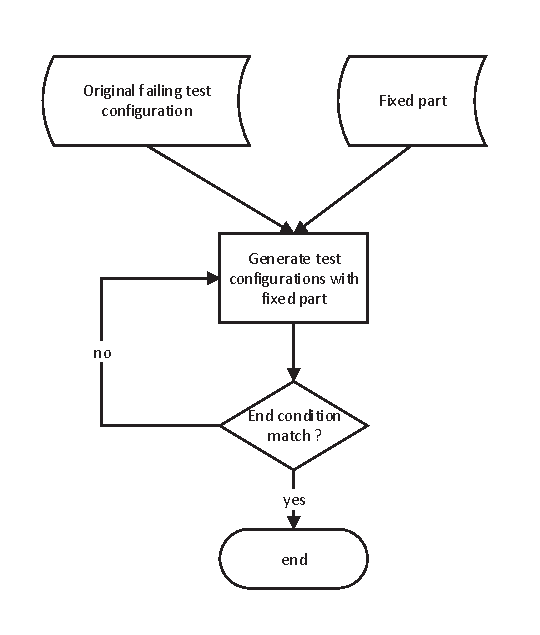
\epsfig{file=framework.eps, height=2.3in}
\caption{the overview of our approach.}
\end{figure}

This figure tell us when given a original failing test configuration and the fixed part, our approach will repeat generating test configurations which mutant the elements in the original test configuration except contain this fixed part until the end condition is matched.



1. Mutant other parts of the original test configurations

2. Execute the SUT under the test configuration make some  according to the result.

original failing test configuration.  and fixed part.

generate test configurations.

judge the based on reuslt

end. regenerate.

In a word, our approach takes a revalidation strategy when encouter different faults until we find a test case. Next we will discuss the two parts in detail.

\subsection{judge the result}
There are three condition we will end our algorithm:

1. If the generated test configuration passed during testing. This means that the fixed part we validated does not contain the failure-inducing elements, so we will send a message to tell the MFS identifying algorithm that this fixed part is a healthy part, and return this passing generated test configuration to these algorithms.

2.If the generated test configuration failed with the same faulty information as the original test configuration.


3.We cannot generate anymore test configurations contained this fixed part and diff from the original test configuration.

In this case, we didn't know which condition does this fixed part should be because we didn't find any test configuration that contain this part and either passed or failed with the same fault information. In this paper, we default set this fixed part as the failure-inducing . And return any test configuration generated.

In fact, to be efficiency, we set the repeat times as a fixed number, say 3 to be end as soon as possible.

Reversely, the only condition that we did not stop is that we encounter a different fault information as the original test configuration, for in that case we did not has enough information whether this fixed part is a failure-inducing part or not as the different fault information may be a masking effect.

\subsection{regenerate}
The regenerate step is to regenerate test configuration that contain the fixed part and does not contain any same elements in the remained part. The reason is that if so we can't not make sure the fixed part or the contained remained part is the failure-inducing part.

Further more, as we having set a fixed number, we can't running all the possible test configuration, so if we did not encounter the passed or the same fault, we will take some more test configuration instead all of them to test. As similar test configuration will trigger the same fault, so we vary them as different as possible to avoid the following condition:

all the regenerated test configuration trigger a fault that have a higher level that the original one.
The method we generate the test configuration it using random method. that is, using random number to take these unfixed part.

We generate as different as possible test cases for the tuple, to avoid some more MFSs that may mask this tuple. To do this we maintain a hash table to record the tuple and its corresponding test cases generated, each time we generate a random test case for this tuple, we will lookup this table to find if this test case is already generated, thus we will avoid generating redundancy test cases.

we will give simple example next to illustrate our approach. Take the fic as a example.

\subsection{simple example}
Assume we have test a system with four parameters, each has three options. And we take the test configuration (0 0 0 0) we find the system encouter a failure called "Err 1". Next we will take the MFS identifying algorithms -- OFOT to identify the MFS for the "Err 1".

The process is listed in table \ref{ofot}. In this table, we can find the algorithm mutant one factor to take the different value from the original test configuration on time. Normally if the test configuration encounter the different condition with the Err 1, OFOT see the MFS was broken, in another word, if we change one factor and it does not trigger the same fault, we will label them as one failure-inducing factor, after we changed all the elements, we will get the failure-inducing schemas. For this case, as when we change the second factor , third factor and the fouth factor, it doesn't trigger the Err 1 ( for second factor, it trigger Err 2 and for the third and fourth, it passed). So finally we can get the MFS --- ( - 0 0 0).

Next, we will check how the ofot works with the assistance of our approach. The process is listed in table \ref{ofot-aug}. We can soon find that the process is very similar to the original ofot algorithm, except that when we change the second factor to generate a new test configuration, we first encounter a new fault Err 2 which is different from the original Err 1, according to our approach, we will eliminate this test configuration and regenerate another one, when we find regenerated test configuration ( 0 2 0 0 ) failed with the same err -- Err 1 with the original test configuration, we stopped the regenerate process for the fixed factor (0 - 0 0), and finally we send this test configuration (0 2 0 0) instead of (0 1 0 0) to the OFOT algorithm, and at last ofot get the more clear and precise MFS for Err 1 --- (- - 0 0).

\begin{table}\renewcommand{\arraystretch}{1.3}
\caption{Identifying MFS using traditional OFOT}
\label{ofot}

\begin{tabular}{|p{0.5\columnwidth}|p{0.3\columnwidth}|} \hline
\bfseries original test configuration & \bfseries fault info \\ \hline
0 \ \ \ \ 0 \ \ \ \  0 \ \ \ \  0  & Err 1
\end{tabular}

\begin{tabular}{|p{0.5\columnwidth}|p{0.3\columnwidth}|} \hline
\bfseries gen test configurations   &\bfseries result \\ \hline
1  \ \ \ \  0 \ \ \ \  0  \ \ \ \  0 & Err 1 \\
0  \ \ \ \  1 \ \ \ \  0  \ \ \ \  0 & Err 2 \\
0  \ \ \ \  0 \ \ \ \  1  \ \ \ \  0 & Pass \\
0  \ \ \ \  0 \ \ \ \  0  \ \ \ \  1 & Pass
\end{tabular}

\begin{tabular}{|p{0.846\columnwidth}|} \hline
\bfseries Mfs identified \\ \hline
(  -  \ \ \  0 \ \ \  0  \ \ \ 0 ) \ \ \ for Err 1 \\
\hline
\end{tabular}
\end{table}



\begin{table}\renewcommand{\arraystretch}{1.3}
\caption{Identifying MFS using OFOT with our approach}
\label{ofot-aug}

\begin{tabular}{|p{0.5\columnwidth}|p{0.3\columnwidth}|} \hline
\bfseries original test configuration & \bfseries fault info \\ \hline
0 \ \ \ \ 0 \ \ \ \  0 \ \ \ \  0  & Err 1
\end{tabular}

\begin{tabular}{|p{0.5\columnwidth}|p{0.3\columnwidth}|} \hline
\bfseries gen test configurations   &\bfseries result \\ \hline
1  \ \ \ \  0 \ \ \ \  0  \ \ \ \  0 & Err 1 \\
\sout{0  \ \ \ \  1 \ \ \ \  0  \ \ \ \  0 } & \sout{Err 2} \\
0  \ \ \ \  2 \ \ \ \  0  \ \ \ \  0 & Err 1 \\
0  \ \ \ \  0 \ \ \ \  1  \ \ \ \  0 & Pass \\
0  \ \ \ \  0 \ \ \ \  0  \ \ \ \  1 & Pass
\end{tabular}

\begin{tabular}{|p{0.846\columnwidth}|} \hline
\bfseries Mfs identified \\ \hline
(  -  \ \ \  - \ \ \  0  \ \ \ 0 ) \ \ \ for Err 1 \\
\hline
\end{tabular}
\end{table}


if the algorithm want to get the result, we will put off the result, and generate another one.

Five setup as follows:

Another note is that:

In detail, for FIC, TRT, OFOT, it can just use the original approach, that it each time test one tuple, and the we use our framework to assign this task.

For CTA, we can use our framework to choose a set of test cases for it to identify the MFS, like shykara do, but different from her work, we just not one test one time, we diff the test cases for different fault.


For SP, we can use our framework for him to generate test cases, it will test multiple tuples one time, and we just first for one fault, then another.

So  our comparison work is just compare the one fault, with a noise for the multiple faults.

\section{empirical studies}
To evaluate our approach, we take two open-source software as our subjects: HSQLDB and Log4j. HSQLDB is a pure-java data-base management software, and Log4j is a logger tool commonly used in java application. Both of them have a large support developers' forum. Furthermore as our approach is a framework that can bee seen as a for the MFS identifying algorithms, so that we afford them five algorithms: fic ofot trt cta sp.

There are three questions we want to figure out from our in this empirical studies:

Q1: does our framework reduce the number of MFSs and the degree of MFS?

Q2: What the real masking state in real softwares.

Q3: does our framework the result is match the result in developer's forum.

\subsection{experiment set up}
We will first model the two objects so that we can use the MFS identifying algorithms. To do this, we first find real faults in the developer's forum, and then read the specification of the software to get the options and its values that can influence its behaviour. The detail of the modeling is listed in table \ref{modelHSQLDB} and table .

\begin{table}\renewcommand{\arraystretch}{1.3}
  \caption{input model of HSQLDB} \centering
  \label{modelHSQLDB}
  \begin{tabular}{p{0.9\columnwidth}}\hline
  \hline
   \bfseries  SQL  properties(TRUE/FALSE)\\
    \hline
    sql.enforce\_strict\_size, sql.enforce\_names,sql.enforce\_refs, sql.enforce\_size, sql.enforce\_types, sql.enforce\_tdc\_delete, sql.enforce\_tdc\_update
  \end{tabular}

  \begin{tabular}{c*{2}{p{0.53\columnwidth}}}
  \hline
  \bfseries table properties &   \bfseries values \\
   \hline
   hsqldb.default\_table\_type & CACHED, MEMORY\\
   hsqldb.tx & LOCKS, MVLOCKS, MVCC\\
   hsqldb.tx\_level & read\_commited, SERIALIZABLE\\
   hsqldb.tx\_level & read\_commited, SERIALIZABLE
  \end{tabular}

  \begin{tabular}{c*{2}{p{0.53\columnwidth}}}
  \hline
  \bfseries Server properties &   \bfseries values \\
   \hline
   Server Type & SERVER, WEBSERVER, INPROCESS \\
    existed form & MEM, FILE
  \end{tabular}

  \begin{tabular}{c*{2}{p{0.53\columnwidth}}}
  \hline
  \bfseries Result Set properties &   \bfseries values \\
   \hline
    resultSetTypes & TYPE\_FORWARD\_ONLY,TYPE\_SCROLL\_INSENSITIVE, TYPE\_SCROLL\_SENSITIVE\\\
    resultSetConcurrencys & CONCUR\_READ\_ONLY,CONCUR\_UPDATABLE \\
    resultSetHoldabilitys & HOLD\_CURSORS\_OVER\_COMMIT, CLOSE\_CURSORS\_AT\_COMMIT
  \end{tabular}

  \begin{tabular}{c*{2}{p{0.53\columnwidth}}}
  \hline
  \bfseries option in test script &   \bfseries values\\
   \hline
   StatementType & STATEMENT, PREPAREDSTATEMENT
  \end{tabular}

\end{table}


Second we will write the test script that can autonomically execute the software according to a given test configuration, furthermore, the test script will collect the executing result. In this paper, we just care two kinds of result: the test script run without any exception and run with triggering exception. For the second result we will distinguish the failure with different exception information.

Third we will take three group experiments, each for the question proposed in the first of this section.

For the first experiment, we will compare the result got by traditional MFS identifying algorithm with the MFS identifying algorithms using our framework. For a particular algorithm, say, OFOT, we will record the number of MFS, the degree of MFSs and the number of test configurations they needed.

The second experiment, we will collect the result got by the algorithms with our framework. Then we will generate a test configuration contain two MFS of the result, and execute to find if one MFS is masked by another. In specific, we will exam every possible pair MFSs, the only constraints is that this two pair MFS must get different fault information.

For the third experiment, we will compare the similarity between the identified result and the result report in the developer's forum. And find whose (traditional or with our framework) result can give more help to the developer of the software.

\subsection{evaluation metrics}
To evaluate the efficiency of our framework, we will compare the results of two approaches. We will count how many MFSs is reduced by our approach and how the degree is reduced by our approach compared to traditional one. This two metric will indicate how much our approach will improve the usability of results.  Additional, we will count how many more test configurations we will generated compare to traditional one, this metric indicate the cost we need over the traditional one.

Then we will exam the result of the algorithm with our framework, to see if any masking is behind them. In detail, we will record how many pair MFS can coexist in a test configuration. And count the privileges of each MFS.

For the third, the similarity is listed as follows:
the followed notation:
Assume we get two schema $S_{A}$,$S_{B}$, the notation$S_{A} \bigcap S_{B}$ indicate the same elements between $S_{A}$ and $S_{B}$. For example $(- 1\ 2 - 3) \bigcap  (- 2\ 2 - 3) = \{ (- - 2 - -) , (- - - - 3)\}$.

\begin{displaymath} Similarity(S_{A},S_{B})= \frac{|S_{A} \bigcap S_{B}|}{\max (Degree(S_{A}),Degree(S_{B})) } \end{displaymath}.

In this formula, the numerator indicate the number of same elements in  $S_{A}$ and $S_{B}$. It is obviously, the bigger the value is the more similar two schemas are.  The denominator give us this information: if the the number of same elements is fixed, the bigger the degree of the schema, the more noise we will encounter to find the fault source. In a word, the bigger the formula can get the better the similarity is between the two schema.

\subsection{result and analysis}

For the second experiment.

\begin{table}
\centering
\caption{Masking effect state}
\label{mask-evluate}
\begin{tabular}{|c|c|c|c| } \hline
all pair & coexisted \& noexised & mask over 6 mfs & over 5 mfs \\ \hline
10 & 5 \& 5 & 3 & 2 \\
\hline\end{tabular}
\end{table}


\section{related works}
combinatorial testing has may factors, Nie give a survey, at some are focus,.

Identify MFS are

then consider the masking effect is , to my best knowledge, only one paper, unfortunately, it just consider the .

Ylimaz propose a work that is feedback driven combinatorial testing, different from our work, it first using CTA classify the possible MFS and then elimate them and generate new test cases to detect possible masked interaction in the next iteration. The difference is that the main focus of that work is to generate test cases that didn't omit some schemas that may be masked by other schemas. And our work is main focus on identifying the MFS and avoiding the masking effect.

\section{Conclusions}
This paragraph will end the body of this sample document.
Remember that you might still have Acknowledgments or
Appendices; brief samples of these
follow.  There is still the Bibliography to deal with; and
we will make a disclaimer about that here: with the exception
of the reference to the \LaTeX\ book, the citations in
this paper are to articles which have nothing to
do with the present subject and are used as
examples only.
%\end{document}  % This is where a 'short' article might terminate

%ACKNOWLEDGMENTS are optional
\section{Acknowledgments}
This section is optional; it is a location for you
to acknowledge grants, funding, editing assistance and
what have you.  In the present case, for example, the
authors would like to thank Gerald Murray of ACM for
his help in codifying this \textit{Author's Guide}
and the \textbf{.cls} and \textbf{.tex} files that it describes.

%
% The following two commands are all you need in the
% initial runs of your .tex file to
% produce the bibliography for the citations in your paper.
\bibliographystyle{abbrv}
\bibliography{sigproc}  % sigproc.bib is the name of the Bibliography in this case
% You must have a proper ".bib" file
%  and remember to run:
% latex bibtex latex latex
% to resolve all references
%
% ACM needs 'a single self-contained file'!
%
%APPENDICES are optional
%\balancecolumns
\appendix
%Appendix A
\section{Headings in Appendices}
The rules about hierarchical headings discussed above for
the body of the article are different in the appendices.
In the \textbf{appendix} environment, the command
\textbf{section} is used to

\subsection{References}
Generated by bibtex from your ~.bib file.  Run latex,
then bibtex, then latex twice (to resolve references)
to create the ~.bbl file.  Insert that ~.bbl file into
the .tex source file and comment out
the command \texttt{{\char'134}thebibliography}.
% This next section command marks the start of
% Appendix B, and does not continue the present hierarchy
\section{More Help for the Hardy}
The sig-alternate.cls file itself is chock-full of succinct
and helpful comments.  If you consider yourself a moderately
experienced to expert user of \LaTeX, you may find reading
it useful but please remember not to change it.
%\balancecolumns % GM June 2007
% That's all folks!
\end{document}
